
%(BEGIN_QUESTION)
% Copyright 2014, Tony R. Kuphaldt, released under the Creative Commons Attribution License (v 1.0)
% This means you may do almost anything with this work of mine, so long as you give me proper credit

Her er en varmeovn på 500 Watt koblet til 230V. 

$$\includegraphics[width=8cm]{i01139x01.eps}$$

Denne ovnen kobles i enden på en lang kabel, som er koblet til 230V. Hver leder i kabelen har en motstand på 3$\Omega$, hvor mye effekt vil oven avgi?

$$\includegraphics[width=15.5cm]{i01139x02.eps}$$

\underbar{file i01139}
%(END_QUESTION)





%(BEGIN_ANSWER)

$P$ = 477.8 Watts

%(END_ANSWER)





%(BEGIN_NOTES)

The purpose of this question, besides providing a good problem-solving exercise for students, is to get them to realize one of the practical implications of power-line resistance.

%INDEX% Electronics review: series and parallel circuits

%(END_NOTES)


